
\documentclass[11pt, titlepage]{article}

% Math text
%\usepackage[utf8]{inputenc}
\usepackage[a4paper,top=2cm,bottom=2cm,left=2cm,right=2cm,marginparwidth=1.75cm,headheight=28pt]{geometry}
%\usepackage[spanish, mexico]{babel}
\usepackage{graphicx}

%\usepackage[utopia]{mathdesign}
\usepackage{amsmath,array}
\usepackage{pdfpages}
% HEADER
\usepackage{fancyhdr,framed}
\setlength{\headheight}{44pt}
\pagestyle{fancy}

% !TeX root = ../main.tex



%% ROCKET
\newcommand{\CG}{{\mathrm{CG}}}
\newcommand{\LCG}{L_\CG}
\def\equilibrium{\mathrm{eq}}


%% DIFFERENTIAL OPERATOR
\makeatletter
\providecommand*{\diff}%
{\@ifnextchar^{\DIfF}{\DIfF^{}}}
\def\DIfF^#1{%
	\mathop{\mathrm{\mathstrut d}}%
	\nolimits^{#1}\gobblespace}
\def\gobblespace{%
	\futurelet\diffarg\opspace}
\def\opspace{%
	\let\DiffSpace\!%
	\ifx\diffarg(%
	\let\DiffSpace\relax
	\else
	\ifx\diffarg[%
	\let\DiffSpace\relax
	\else
	\ifx\diffarg\{%
	\let\DiffSpace\relax
	\fi\fi\fi\DiffSpace}

%% CONTROL:
\newcommand{\dimfont}[1]{\ensuremath{#1}}
\newcommand{\Cme}[1]{\mathbf{#1}}
\newcommand{\Mme}[1]{\mathbf{#1}}
\newcommand{\Nme}[1]{\mathrm{#1}}
\newcommand{\Ts}{T_s}

\newcommand{\eye}{\Mme{I}}
%transpose
\def\dt{\Delta t}
\def\tp{\!^{\top}\!}
% Small
\def\MA{\Mme{A}}
\def\MB{\Mme{B}}
\def\MC{\Mme{C}}
\def\MD{\Mme{D}}
\def\ME{\Mme{E}}

\def\MQ{\Mme{Q}}
\def\MR{\Mme{R}}
\def\MK{\Mme{K}}
\def\MW{\Mme{W}}
\def\MX{\Mme{X}}
\def\MV{\Mme{V}}
\def\ctrb{\Mme{Y}}
\def\Mzero{\Mme{0}}
\def\obsv{\Mme{\mathcal{O}}}

\newcommand{\ts}[2]{\left. #1\right|_{ #2}}

\def\error{\varepsilon}
\def\Cx{\Cme{x}}
\def\Cf{\Cme{f}}
\def\Cy{\Cme{y}}
\def\Cu{\Cme{u}}
\def\Cn{\Cme{n}}
\def\Cd{\Cme{d}}
\def\Czero{\Cme{0}}
\def\Cv{\Cme{v}}
\def\Cz{\Cme{z}}
\def\Cw{\Cme{w}}

\def\Jcost{\Cme{\mathcal{J}}}
% RK4
\def\Ca{\Cme{a}}
\def\Cb{\Cme{b}}
\def\Cc{\Cme{c}}


\def\noise{{n}}
\def\disturb{{d}}
\newcommand{\di}{\ensuremath{\textrm{d}}}

\newcommand{\Matlab}{{\sc Matlab}}

\def\matdiv{\bm{\textbackslash}}

\newcommand{\spartial}[2]{\frac{\partial {#1}}{\partial {#2}}}
\newcommand{\dpartial}[2]{\frac{\partial^2 #1}{\partial #2 ^2}}

%# ROBUST
\def\lap{\mathcal{L}}
\newcommand\lapc[1]{\lap \left\{#1\right\}}
\newcommand\ilapc[1]{\lap^{-1} \left\{#1\right\}}
\def\xbar{\bar{x}}
\def\ubar{\bar{u}} 

\def\MP{\Mme{P}}
\def\ML{\Mme{L}}
\def\MT{\Mme{T}}
\def\MS{\Mme{S}}


\def\Cr{\Cme{r}}
\def\Cn{\Cme{n}}

\def\openloop{{\textrm{\tiny{LA}}}}
\def\closedloop{{ \textrm{\tiny{LC}}}}
\def\true{{ \textrm{\tiny{real}}}}

% RIGID BODY MECHANICS
\newcommand{\frm}[1]{\mathrm{#1}}  % Frame of reference
\newcommand{\ogn}[1]{\mathcal{#1}} % Frame origin / point of reference
\newcommand{\skw}[1]{\tilde{#1}}   % skew matrix notation
\newcommand{\uveci}{{\bm{\hat{\textnormal{\bfseries\i}}}}}
\newcommand{\uvecj}{{\bm{\hat{\textnormal{\bfseries\j}}}}}
\DeclareRobustCommand{\uvec}[1]{{% Unit length vector of arbitrary orientation
		\ifcsname uvec#1\endcsname
		\csname uvec#1\endcsname
		\else
		\bm{\hat{\mathbf{#1}}}%
		\fi
}}
\DeclareRobustCommand{\avec}[1]{{%
		\underline{#1} %		\bm{\mathbf{#1}}%
}}
\DeclareRobustCommand{\bvec}[1]{{% Orthogonal basis vector
%		\ifcsname bvec#1\endcsname
%		\csname bvec#1\endcsname
%		\else
		\bm{\hat{\mathbf{#1}}}%
%		\fi
}}
\def\tform{\mathbf{A}}
\newcommand{\transform}[1]{\tform^\frm{#1}}
\newcommand{\dottransform}[1]{\dot{\tform}^\frm{#1}}
\def\attitude{\mathbf{H}}
\newcommand{\inertia}[2]{J_{\ogn{#1}}^{\frm{#2}}}
\newcommand{\inertiarotor}[2]{\inertia{\!\mathrm{r}#1}{#2}}


\makeatletter
\newcommand*\bigcdot{\mathpalette\bigcdot@{.5}}
\newcommand*\bigcdot@[2]{\mathbin{\vcenter{\hbox{\scalebox{#2}{$\m@th#1\bullet$}}}}}
\makeatother

% THEOREMS/ EXERCISES
\usepackage{amsthm}
\theoremstyle{definition}
%\newtheorem{definition}{Definition}[chapter]
%\newtheorem{theorem}{Teorema}[chapter]
%\newtheorem{exercise}{Ejercicio}[chapter]


\lhead{ Patricio Whittingslow}
\newcommand{\mldivide}{\,{\boldsymbol{\backslash}}\,}


\begin{document}
\begin{titlepage}
	
	\centering
	{\small LIA Aerospace \par}
	
	
	\vspace{8cm}
	{\Huge 2D VTVL rocket simulation using SIMULINK \par}
	\vspace{2cm}
	{ \large {
			Patricio Whittingslow \par}}
	\vspace{4cm}
	\today
	
\end{titlepage}
	
	\section{1D proof of concept using Simulink}
	We begin with the fundamental equations of nonrelativistic motion.
	
	\begin{align}
		F_{\text{total}} &= m\ddot{x} \\
		\dot{x} &= \int \ddot{x} \\
		x &= \int \dot{x}
	\end{align}
	
Our 1D rocket is subject to three forces, \textbf{thrust}, \textbf{drag} and \textbf{gravity}.
\newcommand{\Isp}{I_{sp}}
 We consider gravity ($mg$ where $m = m_{\text{propellant}}+m_{\text{empty}}$) to act on the center of mass which is always aligned at the center of the rocket being a simple 1D case. Mass will vary in time given the rocket is using up propellent to acquire thrust
 
Thrust will be written as $F$ and will be related to the propellent mass by
 \begin{equation}
m_{\text{propellant}} = m_{\text{initial propellant}} - \int  \frac{F}{\Isp}
\end{equation}
where $\Isp$ is the specific impulse of the fuel in Newton-seconds-per-kilogram.
Drag shall be
\[
F_D = \rho C_D A \dot{x}^2
\] 
where $A$ is the area of the rocket facing headwind and $C_D$ is the drag coefficient.

To take into account drag force acts in opposite direction of the velocity it is multiplied by the negative of the sign function of the velocity.

The following two pages include control system for the general system and the engine system.

\includepdf[page=1,angle=90]{OverviewSystem.pdf}
\includepdf[page=1,angle=90]{engineSystem.pdf}

\clearpage
\section{2D model}
\newcommand{\CG}{{\mathrm{CG}}}
\newcommand{\LCG}{L_\CG}
\begin{figure}[htb!]
	\centering
	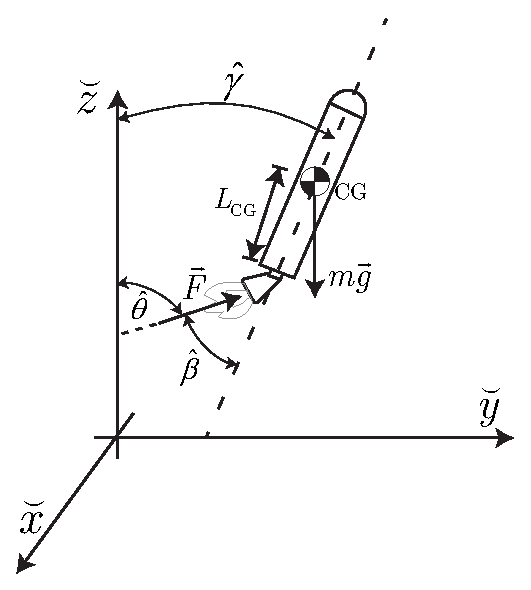
\includegraphics[width=9cm]{fig/rocketFBD.eps}
	\caption{Free Body Diagram for 2D rocket}
\end{figure}

\subsection{Mathematical modeling}
We start by stating the equations of motion of a 2D rocket with angular control over thrust.

\[
\left\{
\begin{array}{l}
	\ddot{y}=\frac{F}{m} \sin(\gamma+\beta) \\
	\ddot{z}=\frac{F}{m} \cos (\gamma+\beta)-g \\
	\ddot{\gamma} = \frac{L_{\CG}\cdot F}{I_{xx}}\sin\beta
\end{array}
\right.
\]
where \(\LCG\) and \(F\) are a function of time, $m =m_0 - \int \dot{m} $ and $\theta = \gamma+\beta$. 

It is worth clarifying the following will not be taken into account:
\begin{itemize}
	\item Air resistance (drag force)
	\item Wind effects
	\item Fuel sloshing
	\item Relativistic effects
\end{itemize}

We then linearize the equations around a stable operating zone, \textbf{a vertical, still rocket}.\footnote{Modifications to system will need to be made if rocket is to be an orbital delivery device.} This way  small angle relations will be a reasonable approximation.

System linearization around steady point:
\begin{align*}
	\gamma^* = 0 \\
	\beta^* = 0 \\
	F^* = mg
\end{align*}
this way our state space variable for $F$ will be the deviation or peturbation from the steady point. From now on $\Delta F = F- mg$
\subsection{State space representation}
It follows that the number of state-space variables be equal to the number of independent energy storage elements. These are as follows

\begin{enumerate}
	\item[$z$] Gravitation potential energy
	\item[$\dot{y},\dot{z}$] Kinetic energy of rocket
	\item[$\dot{\gamma}$] Angular momentum of rocket
\end{enumerate}
thus, state-space variables are chosen as follows
\begin{align*}
	x_1 = y \\
	x_2 = \dot{y} \\
	x_3 = z \\
	x_4 = \dot{z} \\
	x_5 = \gamma \\
	x_6 = \dot{\gamma}
\end{align*}
where $\dot{x_1} = x_2$, $\dot{x_3} = x_4$ and $\dot{x_5} = x_6$

Let us recall the following Taylor expansion for linearization of trigonometric expressions.
\[
\sin(x+y)|_{x=x_0+\Delta x,y=y_0+\Delta y} \approx \sin(x_0+y_0) + \cos(x_0 + y_0) (x-x_0) + \cos(x_0 + y_0) (y-y_0)
\]
The linearized dynamic equation of the second, third and fourth state are given by the equations of motion mentioned at the start of this document. Below are all the state equations
\begin{equation}
	\dot{x_2} = \frac{F}{m} \left( \gamma+\beta \right) = g x_5 + g u_2 
\end{equation}
\begin{equation}
\dot{x_4} = \frac{F}{m} - g =\frac{F-F_0}{m}= \frac{u_1}{m}
\end{equation}
\begin{equation}
\dot{x_6} = \frac{\LCG \cdot F}{I_{xx}} \beta = \frac{\LCG \cdot mg}{I_{xx}} u_2 
\end{equation}

where $\Ts$ is the sampling time.

The input and output vectors are 
\[
\Cme{u}(t) = \begin{bmatrix}
u_1 \\
u_2
\end{bmatrix} = \begin{bmatrix}
\Delta F \\
\beta
\end{bmatrix}
\]
\[
\Cme{y}(t) = \begin{bmatrix}
y_1 \\
y_2 \\
y_3
\end{bmatrix} = \begin{bmatrix}
y \\
z \\
\gamma
\end{bmatrix}
\]
such that the output equations are

\begin{equation}
	y_1 = x_1 
\end{equation}
\begin{equation}
	y_2 = x_3
\end{equation}
\begin{equation}
	y_3 = x_5
\end{equation}

The matrices are then written ($\Mme{D} = [0]$)
\begin{equation} \label{eq:ssmatrices}
	\Mme{A} = 
	\left[\begin{array}{cccccc} 0 & 1 & 0 & 0 & 0 & 0\\ 0 & 0 & 0 & 0 & g & 0\\ 0 & 0 & 0 & 1 & 0 & 0\\ 0 & 0 & 0 & 0 & 0 & 0\\ 0 & 0 & 0 & 0 & 0 & 1\\ 0 & 0 & 0 & 0 & 0 & 0 \end{array}\right],\quad \Mme{B} = 
	\left[\begin{array}{cc} 0 & 0\\ 0 & g\\ 0 & 0\\ \frac{1}{m} & 0\\ 0 & 0\\ 0 & \frac{\LCG \cdot mg}{I_{xx}} \end{array}\right], \quad \Mme{C} =  \left[\begin{array}{cccccc} 1 & 0 & 0 & 0 & 0 & 0\\ 0 & 0 & 1 & 0 & 0 & 0\\ 0 & 0 & 0 & 0 & 1 & 0 \end{array}\right]
\end{equation}

\subsection{Control System Design}
The system shown in \eqref{eq:ssmatrices} is fully state controllable.

\end{document}
\clearpage

%\newcommand{\dimfont}[1]{\ensuremath{#1}}
%\newcommand{\Cme}[1]{\mathbf{#1}}
%\newcommand{\Mme}[1]{\mathbf{#1}}



\section{Control theory}
\subsection{Basics}
Taylor expansion (Linearization) of two-variable nonlinear equation.
\[
f(x,y) = f(\overline{x},\overline{y}) + \left[ \frac{\partial f}{\partial x} (x-\overline{x}) +\frac{\partial f}{\partial y} (y-\overline{y}) \right] + \ldots
\]


Matlab command to convert state space to transfer function \verb|[num,den]=ss2tf(A,B,C,D,iu)| where \verb|iu| must be specified for systems with more than one input.








\subsection{State space}
\(\Cme{u}(t)\) is inputs vector and is of size \(\dimfont{q\times 1}\) for a given system, i.e: \( \Cme{u}(t)=\begin{bmatrix}
u_1 \\ u_2
\end{bmatrix}\) for two input system, \(\dimfont{q}=2\).

\(\Cme{y}(t) \) is the output vector of size  \(\dimfont{r\times 1}\). 

Thus we define the \textbf{state space variables} so that system output is purely in function of current system state variables and input variables.
\[
\text{System Output} = f\left( \text{Current System State, System Input} \right)
\]

We will define \(X\) or \(\Cme{x}\) as our system state variables. There are some important aspects to note about state space variables such as
\begin{itemize}
	\item System output \(\Cme{y}(t)\) will be a function of them
	\item They change over time
	\item They are internal to the system
	\item They may include system outputs (outputs will be a function of themselves in part)
	\item Their selection is inherent part of the system design process and there are different methods of selecting them.
	\item We will assume there is a minimal quantity of state variables that is sufficient to accurately describe the system
	\item If all system inputs \(u_j\) are defined beforehand for \(t\geq t_0\) then \(\Cme{x}(t)\) defines all system states for time \(t \geq t_0\)
\end{itemize}


The mathematical representation of state space variables will be will be that of the \textbf{state vector} \(\Cme{x}(t)\) of size \(\dimfont{n}\times 1\).

To model our system we then define the equations that govern it in \textbf{state space}\footnote{State space can be thought of an \dimfont{p}-dimensional space whose axes are the state variables (\(x_1,x_2\ldots\))}. These are the \textbf{state-space equations} of the system. For a dynamic system these must include a variable that serves as memory of inputs for \(t \geq t_1\). \textit{Integrators} serve as memory devices for \textit{continuous-time} models, however, our state-space representation is discrete! This is when state-space variables come in handy: The outputs of integrators can be considered as the variables that define the internal state of the dynamic system (Ogata). 


For a system of size \(q=r=n=1\) one has the state-space representation defined as:
\[
\dot{x}(t)=g\left[t_0,t,x(t),x(0),u(t)\right] ,\qquad y=h\left[t,x(t),u(t)\right]
\]

For a \textit{linear} system of arbitrary size it is convenient to represent it in it's linearized form

\begin{equation}
	\Cme{\dot{x}} (t) = \Mme{A}(t) \Cme{x}(t) + \Mme{B}(t) \Cme{u}(t)
\end{equation}
\begin{equation}
\Cme{y} (t) = \Mme{C}(t) \Cme{x}(t) + \Mme{D}(t) \Cme{u}(t)
\end{equation}

where 
\begin{itemize}
	\item[\(\Mme{A}_{\dimfont{n}\times\dimfont{n}}\)] System matrix. Relates future state change with current state. May be zero.
	\item[\(\Mme{B}_{\dimfont{n}\times\dimfont{q}}\)] Control matrix. How system input influences state change. May be zero.
	\item[\(\Mme{C}_{\dimfont{r}\times\dimfont{n}}\)] Output matrix. How system state influences system output.
	\item[\(\Mme{D}_{\dimfont{r}\times\dimfont{q}}\)] Feed Forward matrix. How system input influences system output. Is usually zero.
\end{itemize}
the system is said to be \textbf{time-invariant} if the above matrices are not dependent of time. An example of a \textbf{time-variant} system is a spacecraft, whose mass changes due to fuel consumption.

One method of state space variable selection is \textbf{physical selection}. This method is based on energy acumulators. It can b-e said that \textit{the minimum number of state-space variables needed to model the system accurately is equal to the number of independent energy accumulators.} When state-space variable is not a energy variable it is said to be an augmented variable.





\end{document}